\chapter{Dynamics of Wheeled Mobile Robots }
\label{c4_SenCal}
In the field of mobile robotics, extensive research has been carried out. 
Mobile robots can broadly be divided into three categorises-wheeled robots, legged robots ~\cite{machado2006overview}, and aerial vehicles ~\cite{valavanis2014handbook}. 
There are few mobile robots which use both wheels and legs for locomotion for example, in Creadapt  \cite{mouret2015evolutionary} in order to take advantage of both modes of locomotion. 
Among these the most extensively studied are the  Wheeled Mobile Robots (WMR). 
They have been classified into five generic classes by Champion etal. \cite{campion1996structural},~\cite{campion2008wheeled}  based on there mobility resulting from the kinematic constrains due to  different wheel types.
 The most common among these are the  3 wheeled differential drive WMR with one castor wheel.
  Because of its simplicity in modelling, they have been used in most of the  control and motion planing algorithms  \cite{desantis1995modeling}, \cite{koh1999smooth} and \cite{d1995control}. 

In order to develop a model-based control algorithm it is imperative to have good dynamic model of the WMR.
 These dynamic models are used in  simulation software,  Software in Loop (SIL) testing and Hardware in Loop (HIL) testing  of the controllers.
 Different methods have  been adopted to derive the dynamic model of WMRs.
  A general dynamical model was derived for three-wheel mobile robots with nonholonomic constraints  by B. d'Andrea-Novel \cite{d1991modelling} using  Lagrange formulation.
    Alternatively Thanjavur and Rajagopalan \cite{thanjavur1997ease} has used Kane's method  and  Saha et al. \cite{saha1991dynamics},\cite{saha1989kinematics} used Natural Orthogonal Compliment (NOC) method for the same.  
 
All the papers known to us use the standard caster wheel in deriving the dynamic model of the WMR. In this chapter the modelling is carried out considering the Castor wheel in the most general configuration.
 In the stranded castor wheel configuration the axis of rotation is perpendicular to the line joining the pivot and the axis of rotation, as shown in Figure \ref{fig:std} whereas in this study they are oriented in  the most general way, as shown in figure Figure \ref{fig:gen}. 
 The concept of the NOC which here inherently takes into account the non-holonomic constraint of the wheels has been used.
  Moreover, being a matrix based approach, it is convenient for numerical simulations. 
\section{Modeling using the Natural Orthogonal Compliment (NOC)}
Let us consider a system $n$ rigid bodies interconnected with different types of joints. 
Let $f_i$ be the net force acting at the center of mass (CM) of the $i-th$  body and $n_i$ is the net moment.
 If $m_i$ is the mass, $I_{ci}$ is the  moment of inertia with respect to the CM, $c_i$ is the position vector of the CM and $\omega_i$ is the angular velocity of the same body, then equation of motion of the $i-th$ rigid body is given by Newton-Euler equations as 
\begin{equation}
\label{NE}
f_i=m_i\ddot{c_i} \quad and \quad n_i=I_{ci} \omega_i+\omega_i \times I_{ci} \omega_i
\end{equation}
Let us  define twist ($t$) and wrench($w$) as 
\begin{equation*}
t_i \equiv \begin{pmatrix}
\omega_i\\ \dot{c_i}
\end{pmatrix} \quad
w_i \equiv \begin{pmatrix}
n_i\\f_i
\end{pmatrix}
\end{equation*}
Note that the wrench $w_i$ acting on the $i-th$ body can be decomposed into $w^w_i$, called the \textit{working component} and  $w^C_i$, the \textit{non-working component}.
 The working component consists of all the external  forces and torques, which imparts/extracts energy to/from the system, e.g. motor actuating torque.
  The non-working component of the wrench consists of the forces and torques that are used to constrain the motion of the body at the joints.
Then, Newton-Euler equation (\ref{NE}) can be rewritten  in a single matrix equation as 
\begin{equation}
\label{2}
M_i\dot{t_i}+W_iM_it_i=w^w_i+w^c_i \quad \because w_i \equiv w^w_i+w^c_i
\end{equation}
where
\begin{equation}
\label{3}
M_i \equiv \begin{pmatrix}
I_{ci} & 0\\0 & m_i\tilde{1}
\end{pmatrix} ,
\quad W_i\equiv \begin{pmatrix}
\Omega_i &0\\0&0
\end{pmatrix},
\quad
\Omega_i\equiv \omega_i\times \tilde{1}
\end{equation}
in which  $\omega_i\times 1$, is refered as the crossproduct matrix of vector $\omega_i$ and $\tilde{1}$ denotes the identity matrix.
For details, refer to \cite{angeles2013fundamentals},\cite{saha2010robotics}.


If we define \[M \equiv diag[M_1,M_2,...M_n[, \quad W \equiv diag[W_1,W_2,...W_n], \quad t \equiv [t_1^T,t_2^T, ....t_n^T]^T\] and 
\[ w^j \equiv [{w_1^j}^T,{w_2^j}^T, ....{w_n^j}^T]^T, \,j=c,w \]
Then the equation of all the $n$ rigid bodies in the system can be collected and written as a single matrix equation as 
\begin{equation}
\label{DCE}
M\dot{t}+WMt=w^c+w^w
\end{equation}
 The above equation is referred to as  decoupled equations of motion of the system.



The kinematic constraints both holonomic and non-holonomic (e.g. pure rolling) between two bodies $i$ and $j$ of a system can be expressed as linear homogeneous system of algebraic equations \cite{angeles2013fundamentals}, namely 
\begin{equation}
A_it_i+A_jt_j=0
\end{equation}
where $A_i,A_j$ depend on the kinematic parameters.

The constraint equations corresponding to all the joints in the system can be written in terms of the \textit{generalized twist vector} $t$. Furthermore if, $ \dot{\theta} \equiv(\dot{\theta_1},\dot{\theta_2},....)^T$ denote the \textit{independent generalized joint rates}, one can then write $t$ in terms of $\dot{\theta}$ as $t=T\dot{\theta}$. 
Using the fact, that $\dot{\theta}$ can take any arbitrary value, we get
\begin{equation}
\label{AT}
At=0 , \quad \Rightarrow  AT\dot{\theta}=0\quad \Rightarrow AT=0
\end{equation}
The above equation (\ref{AT}) indicates that $T$ is the orthogonal compliment of $A$.
 Since this relation arises naturally, hence the name \textit{Natural Orthogonal Complement}.
  It can be shown \cite{angeles2013fundamentals} that the non-working wrench $w^c$ lies in the range space of $A^T$.
   In view of equation \ref{AT}, it can also be proved that $w^c$ lies in the null space of $T^T$, therefore
\begin{equation}
T^Tw^c=0
\end{equation}
To eliminate the non-working forces and moments, i.e. $w^C$ from the uncoupled equation of motion (\ref{DCE}), we multiply both sides of the equation  by $T^T$,
\begin{equation}
 T^TM\dot{t}+T^TWMt=T^Tw^W, \quad
 \Rightarrow T^TMT\ddot{\theta}+T^T(M\dot{T}+WMT)\dot{\theta}=T^Tw^T
 \label{eqn:CEM}
\end{equation}
Equation \ref{eqn:CEM} represents the dynamic equation of  interconnected $n$-body system.
 This equation is expressed in terms of the independent generalized joint rates $\dot{\theta}$ and cosponsoring  acceleration $\ddot{\theta}$. Further. using the relations $t=T\dot{\theta}$ and $\dot{t}=\dot{T}\dot{\theta}+T\ddot{\theta}$  in equation \ref{eqn:CEM}  the final equations of motion can be written as

\begin{equation}
\label{CE}
 \quad I(\theta)\ddot{\theta}=C(\theta,\dot{\theta})\dot{\theta}+\tau
\end{equation}
where
\[I(\theta)\equiv T^TMT\quad :\text{generalized inertia matrix}\]
\[C(\theta,\dot{\theta})\equiv -T^T(M\dot{T}+WMT)\dot{\theta} \quad :\text{generalized matrix of convective inertia terms}\]
\[\tau\equiv T^Tw^T \quad :\text{ generalized vector of driving forces }\]


\begin{figure}
	\begin{minipage}[t]{0.5\textwidth}
	\centering
		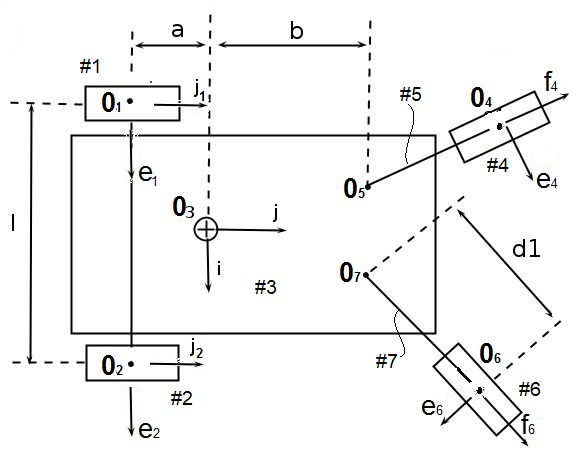
\includegraphics[width=3in]{Chapter4/fig/fig1.jpg} 
		\caption{WMR-Std. Castor}\label{fig:std}
	\end{minipage}
	\hfill
	\begin{minipage}[t]{0.5\textwidth}
	\centering
		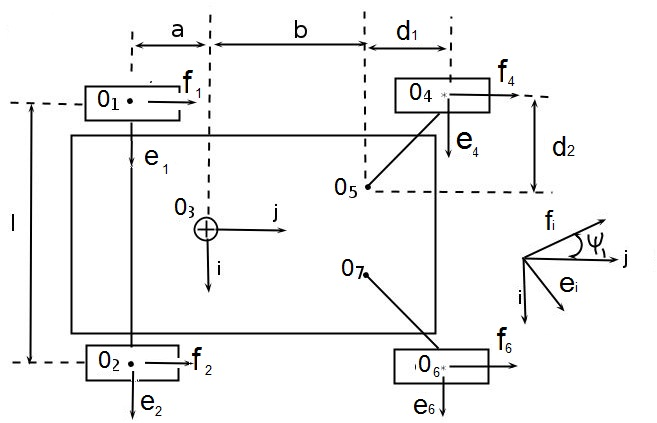
\includegraphics[width=3.5in]{Chapter4/fig/fig2.jpg} 
		\caption{WMR-general}\label{fig:gen}
			\end{minipage}
\caption{Castor wheel configuration of a WMR}
\end{figure}


\section{Dynamic Equation of WMR}
The dynamic equation of a differentially driven 3 wheeled mobile robot based on the  Natural Orthogonal Compliment (NOC) has been presented by Saha~\cite{saha1991dynamics}. The vehicle consisted of 2 driven wheel and one standard caster wheels. In general, for large vehicles, it necessary to have at least four wheels from the point of stability of the vehicle. Such a vehicle is shown in figure \ref{fig:std}. It may be noted that the caster wheels used in this case are the standard caster wheel configuration, where the angle between line $O_4O_5$ and vector $e_4$ is  $90\deg$. Which is a special case of the more general configuration of the caster wheels shown in figure \ref{fig:gen}, where angle between line $O_4O_5$ and vector $e_4$ is not $90\deg$

 The vehicle considered for analysis in this chapter is shown in figure \ref{fig:gen}. It consists of two independently driven wheels at the back and two generalized caster wheels at the front. The actuated wheels are labelled as body \#1 and \#2. The platform is body \#3. The first caster wheel and its bracket is labelled as \#4 and \#5 respectively, with the castor pivoted at $O_5$. Similarly the second castor is pivoted at $O_7$, and its bracket and wheel is labelled as \#6 an \#7 respectively, all the wheels are assumed to be rolling without slipping.  
\subsection{Kinematic analysis}
In order to proceed with the kinematic analysis of the vehicle in figure \ref{fig:gen}, we define a orthogonal triad of vectors ${i,j,k}$ at point $O_3$, the control point of the platform, as shown in the figure. If $\dot{\theta_1}$ and $\dot{\theta_2}$ \footnote{ positive when pointing along $i$} denote the rates of rotation of wheel \#1 and \#2 then the linear velocity of points $O_1$ \& $O_2$ under pure rolling condition is given by 
\begin{equation}
\label{velO1}
\bm{\dot{o_i}}=r\dot{\theta_i}j, \quad \text{r=radius of wheel}
\end{equation}
The angular velocity of the platform $\omega_3$ can be written as 
\begin{equation}
\label{omegaPlat}
\bm{\omega_3}=(r/l)(\dot{\theta_1}-\dot{\theta_2})\bm{k}
\end{equation}
Further, the velocity of point $O_3$ can be written as
$\bm{\dot{o_3}=\dot{o_i}+\omega_3 \times (c-o_i)}, \quad i=1,2$. Where $o_3 $ and $o_i$  is the position vector of points $O_3$ and $O_i$ respectively, with respect to some  point fixed to the ground. By eliminate $\omega_3$  we get the following:
\begin{equation}
\label{velPlat}
 \quad \quad \bm{\dot{o_3}}=[(ar/l)(\dot{\theta_1}-\dot{\theta_2})+(r/2)(\dot{\theta_1}+\dot{\theta_2})]\bm{i}
\end{equation}

Now, the angular velocity of the drive wheel \#1 can be expressed as $\bm{\omega_1}=-\dot{\theta_1}i+\omega_3k$. Using equation \ref{omegaPlat}, the same can be rewritten as 
\begin{equation}
\label{omegaWheel1}
\bm{\omega_1}=\begin{pmatrix}
-i+(r/l)k & -(r/l)k
\end{pmatrix}
\begin{pmatrix}
\dot{\theta_1}\\\dot{\theta_2}
\end{pmatrix}
\end{equation}
Based on  equations \ref{velO1} and \ref{omegaWheel1}, we can write the twist for wheel \#1 in terms of $\dot{\theta_a}\equiv (\dot{\theta_1},\dot{\theta_2})^T$, as 
\begin{equation}
\label{twist1}
t_1=\begin{pmatrix}
\omega_1\\\dot{o_1}
\end{pmatrix}=
\begin{pmatrix}
-i+(r/l)k & -(r/l)k\\ rj & 0
\end{pmatrix}
\begin{pmatrix}
\dot{\theta_1}\\\dot{\theta_2}
\end{pmatrix}
\end{equation}

Similarly, for the other actuated wheel \#2, one get

\begin{equation}
\label{twist2}
t_2=\begin{pmatrix}
\omega_1\\\dot{o_1}
\end{pmatrix}=
		\begin{pmatrix}
		-i+(r/l)k & -(r/l)k\\  0 &rj
		\end{pmatrix}
		\begin{pmatrix}
		\dot{\theta_1}\\\dot{\theta_2}
		\end{pmatrix}\\
		\end{equation}

To calculate the twist, $t_3$ of the platform body \#3, equation \ref{omegaPlat} and \ref{velPlat} are combined to get
\begin{equation}
\label{twist3}
t_3=\begin{pmatrix}
\omega_3\\\dot{o_3}
\end{pmatrix}=
\begin{pmatrix}
\rho\delta & -\rho\delta\\
r(\lambda i+(1/2)j) & r(-\lambda i+(1/2)j)
\end{pmatrix}
\begin{pmatrix}
\dot{\theta_1}\\\dot{\theta_2}
\end{pmatrix}
\end{equation}
where
\[ \delta\equiv d/l, \quad \rho \equiv r/d, \quad \lambda \equiv a/l \]

From the above three equations we get 
$T_1=\begin{pmatrix}-i+(r/l)k & -(r/l)k\\ rj & 0\end{pmatrix}$,   
$T_2=\begin{pmatrix}	-i+(r/l)k & -(r/l)k\\  0 &rj \end{pmatrix}$, $T_3=\begin{pmatrix}
	\rho\delta & -\rho\delta\\
	r(\lambda i+(1/2))j & r(-\lambda i+(1/2))j
	\end{pmatrix}$


In order to calculate the twist of the caster bracket and the caster wheel, we need to express the  unactuated joint rates, $\dot{\psi_1}$ and $\dot{\phi_1}$, in terms of the actuated joint rate vector $\dot{\theta_a}$. note here that $\dot{\psi_1}$ denotes the rate of rotation of bracket body \#5 about $O_5$ with respect to the platform, and 
$\dot{\phi_1}$ the rate of rotation of caster wheel body \#4 about its axis $e_4$ with respect to bracket. The velocity of $O_5$ can be expressed in two independent forms,namely, one in terms of the velocity of $O_3$ and the other one in terms of the velocity of $O_5$, i.e.,
\begin{equation}
\dot{o_5}=\dot{o_4}+\omega_5\times(d_1e_4-d2f_4), \quad
\dot{o_5}=\dot{o_4}+\omega_5\times(d_1e_4-d2f_4)
\end{equation}
On equating the above two equations together, and using the rotation matrix between coordiante system $\{i,j,k\}$ and $\{e_4,f_4,k\}$, to express the equation in $e_4$ and $f_4$, we get
\begin{equation}
(-\dot{\phi_1}r+\dot{\psi_1}d_1)f_3+d_3\dot{\psi_1}e_3=\dot{o_3}
+\omega_3(m\cos\psi_1-b\sin\psi_1-d_1)e_4
\end{equation} 
Taking the dot product of the above equation first with $e_4$ and then with $f_4$, and using equation \ref{velPlat} for $\dot{o_3}$, we get
\begin{eqnarray}
\label{unac2act1}
\begin{pmatrix}
d_2&0\\-d_1 &r
\end{pmatrix}
\begin{pmatrix}
\dot{\psi_1}\\ \dot{\phi_1}
\end{pmatrix}
&=&\begin{pmatrix}
(-ar/l)S_{\psi_1}+(r/2)C_{\psi_1}+\delta_1 & 
(ar/l)S_{\psi_1}+(r/2)C_{\psi_1}-\delta_1 \\
(ar/l)C_{\psi_1}+(r/2)S_{\psi_1}+\delta_2 & 
(-ar/l)C_{\psi_1}+(r/2)S_{\psi_1}-\delta_2 
\end{pmatrix}\dot{\theta_a}\nonumber \\
&=&[F_{ij}]\dot{\theta_a}
\end{eqnarray}
where, 
\[ \delta_1=(r/l)(mC_{\psi_1}-bS_{\psi_1}-d2, \quad  \delta_2=(r/l)(mS_{\psi_1}+bC_{\psi_1}+d_1) \]

Similarly, for the other caster wheel we get,
\begin{align}
\label{unac2act2}
\begin{pmatrix}
d_2&0\\-d_1 &r
\end{pmatrix}
\begin{pmatrix}
\dot{\psi_2}\\ \dot{\phi_2}
\end{pmatrix}
&=\begin{pmatrix}
(-ar/l)S_{\psi_2}+(r/2)C_{\psi_2}-\delta_3 & 
(ar/l)S_{\psi_2}+(r/2)C_{\psi_2}+\delta_3 \\
(ar/l)C_{\psi_2}+(r/2)S_{\psi_2}+\delta_4 & 
(-ar/l)C_{\psi_2}+(r/2)S_{\psi_2}-\delta_4 
\end{pmatrix}\dot{\theta_a}\nonumber \\
&=[G_{ij}]\dot{\theta_a}
\end{align}
where, 
\[ \delta_3=(r/l)(mC_{\psi_2}+bS_{\psi_2}+d2, \quad  \delta_4=(r/l)(mS_{\psi_2}+bC_{\psi_2}+d1 \]




 The angular and the liner velocity of the CM of the caster wheel,\#4 is  written in-terms of the co-ordinate frame fixed to the bracket \#5, i.e. $\{e_4,f_4,k\}$, as
\begin{equation}
\label{omegacastor1}
\omega_4=\dot{\phi_1}e_4+(\omega_3+\dot{\psi_1})k, \quad
\dot{o_4}=\dot{\phi_1}e_4
\end{equation}
Using equations \ref{unac2act1} and \ref{omegaPlat}, the twist $t_4$ can be written as
\begin{equation}
\label{twist4}
t_4=\begin{pmatrix}
\Theta_4\\C_4
\end{pmatrix}\dot{\theta_a}
\end{equation}
Using the definition of $F(i,j)$ in  equation \ref{unac2act1}, $\Theta_4$ and $C_4$ can be written as 
\[ \Theta_4=[F_{11}e_4+\bar{F_{21}}k \quad F_{12}e_4+\bar{F_{22}}k],\quad 
C_4=r[-F_{11}f_4 \quad -F_{12}f_4]\]
\[\bar{F_{21}}=F_{21}+\rho \delta, \quad \bar{F_{22}}=F_{22}-\rho\delta\]

The angular and the liner velocity of the CM of the caster bracket\#5  expressed in the co-ordinate frame fixed to the bracket is given by
\begin{equation}
\omega_4=\dot{\phi_1}e_3+\dot{\psi_1}k, \quad
\dot{o_4}=\dot{o_4}+\omega_5\times [-df_3]
\end{equation}
Using equations   \ref{omegaPlat} \& \ref{unac2act2}, the twist $t_5$ can be written as
\begin{equation}
\label{twist5}
t_5=\begin{pmatrix}
\Theta_5\\C_5
\end{pmatrix}\dot{\theta_a}
\end{equation}
where
\[ \Theta_5 \equiv [\bar{F_{21}}k \quad \bar{F_{22}}k],\quad 
C_5\equiv d[(1/2)\bar{F_{21}}e_4-\rho F_{11}f_4 \quad (1/2)\bar{F_{22}}e_4-\rho F_{12}f_4]\]
In a similar manner, the twist $t_6$ and $t_7$  of the other caster wheel and its bracket can be written as 
\begin{equation}
\label{twist6}
t_6=\begin{pmatrix}
\Theta_6\\C_6
\end{pmatrix}\dot{\theta_a}, \quad t_7=\begin{pmatrix}
\Theta_7\\C7
\end{pmatrix}\dot{\theta_a}
\end{equation}
Using  $G(i,j)$ defined in  equation \ref{unac2act2}, $\Theta_6$, $C_6, \Theta_7$ and $C_7$ can be written as 
\[ \Theta_6 \equiv [G_{11}e_6+\bar{G_{21}}k \quad G_{12}e_6+\bar{G_{22}}k],\quad 
C_6 \equiv r[-G_{11}f_6 \quad -G_{12}f_6]\]
\[ \Theta_7 \equiv [\bar{G_{21}}k \quad \bar{G_{22}}k],\quad 
C_7 \equiv d[(1/2)\bar{G_{21}}e_6-\rho G_{11}f_6 \quad (1/2)\bar{G_{22}}e_6-\rho G_{12}f_6]\]
\[\bar{G_{21}} \equiv G_{21}+\rho \delta, \quad \bar{G_{22}}\equiv G_{22}-\rho\delta\] 

\subsection{Dynamic equations}
Based on the twist calculated in terms of the independent joint rate vector vector $\dot{\theta_a}$, we now derive the generalized inertia matrix and the matrix of convective inertia term for the coupled equation of motion \ref{CE}.
\subsubsection{Generalized Inertia Matrix, $I$}
 The above equations gives the twist of individual body, i.e $t_i=T_i\dot{\theta_a}$. As defined earlier  $t=[t_1^T, t_2^T....t_7^T]^T$ and $t=T\theta$ we get  \[T=[T_1^T, T_2^T,... T_7]^T\] Since the matrix $M$ is block diagonal, the inertia matrix of the full system is given by
\begin{equation}
I=T^TMT=T_1^TM_1T_1+T_2^TM_2T_2+...T_7^TM_7T_7
\end{equation}
We define the contribution of rear wheels alone to the inertia matrix by $I_m$ as  \[ I_m=\sum_{i=1,2}T_i^TM_iT_i\] then
\begin{equation}
\label{eqn:I_wheel}
I_m=\begin{pmatrix}
I_w+(\rho\delta)^2H++m_wr^2 & -2(\rho\delta)^2H
\\
-2(\rho\delta)^2H &I+(\rho\delta)^2H++m_wr^2
\end{pmatrix} 
\end{equation}
where $ M_i \equiv\begin{pmatrix}
\tilde{I_w} &0\\0 & m_w\mathbf{1}
\end{pmatrix} $ and $\tilde{I_w}\equiv\begin{pmatrix}
I_w&0&0\\0&H&\\0&0&H
\end{pmatrix}$. Matrix $\tilde{I_w}$ is the $3\times 3$ moment of inertia matrix of the wheel in co-ordinate frame $\{i,j,k\}$, mass of the motorized wheels is  $m_w$ and $mb{1}$ is the $3\times 3$ identity matrix.
If the mass of the platform is $m_p$ and its moment of inertia about vector ${k}$ is $I_p$, then as derived in \cite{angeles2013fundamentals} 
\begin{equation}
\label{eqn:I_platform}
I_3=T^T_3M_3T_3 =I_p(\rho\delta)^2\begin{pmatrix}
1&-1\\-1&1 \end{pmatrix}\\
+m_pr^2\begin{pmatrix}
(1/4)+\gamma^2 & (1/4)-\gamma^2\\(1/4)-\gamma^2 & (1/4)+\gamma^2
\end{pmatrix}
\end{equation}
Similarly, if $m_c$ is the mass of the castor wheel and it is assumed to be a solid disk, then the generalized inertia matrix  can be written as
\begin{align}
I_c=\sum_{i=4,6}T^T_iM_iT_i=(m_cr^2/4)&
\begin{pmatrix}
6F_{11}^2+\bar{F_{21}}^2 & 6F_{11}F_{12}+\bar{F_{21}}\bar{F_{22}}\\
6F_{11}F_{12}+\bar{F_{21}}\bar{F_{22}} & 6F_{12}^2\bar{F_22}
\end{pmatrix}\\ \nonumber
&+\begin{pmatrix}
6G_{11}^2+\bar{G_{21}}^2 & 6G_{11}G_{12}+\bar{G_{21}}\bar{G_{22}}\\
6G_{11}G_{12}+\bar{G_{21}}\bar{G_{22}} & 6G_{12}^2\bar{G_22}
\end{pmatrix}
\end{align}
If the mass of the brackets, i.e., body \#5 and \#7, are small compared to the mass of the caster wheels, then the contribution of $T^T_5M_5T_5$ and $T^T_7M_7T_7$ can be neglected.


\subsubsection{Matrix of Convective Inertia term $C$}
The matrix of convective inertia terms of equation \ref{CE} can be broken down into two parts, $T^TM\dot{T}$ and $T^TWMT$.  As given in equations \ref{twist1}, \ref{twist2} and \ref{twist3} $T_1,T_2,T_3$ of the rear wheels and the platform is constant. Therefore $T^TM\dot{T}=0$. The generalized inertia matrix too is constant for the rear wheels and the platform, so the vector $I_i\omega_i$ is parallel to vector $\omega_i, i=1..3$ $\rightarrow\omega\times I\omega=0$ $\rightarrow T^TWMT =0$. This shows that contribution of the rear wheels and the platform  to the convective inertia term is zero. Moreover we have considered the mass of the brackets to be zero, so they also do not contribute to the convective inertia term. Hence
\begin{equation}
\label{Convective}
C=T^TM\dot{T}+T^TWMT=\sum_{i=4,6}T^T_iM_i\dot{T_i}+\sum_{i=4,6}T_i^TW_iM_iT_i
\end{equation}
The expression for the first term is found by using equations \ref{unac2act1}, \ref{unac2act2}, \ref{twist4} and \ref{twist6}. The terms $\dot{F_{ij}}$ and $\dot{G_{ij}}$ denote the derivatives of the elements of the matrix $F$ and $G$ defined in \ref{unac2act1}, \ref{unac2act2} . To find $\dot{T_4}$ and  $ \dot{T_6}$ we have used the fact $\dot{e_4}=\omega_4 \times e_4 $ and $\dot{e_4}=\omega_6 \times e_6 $. 
\begin{equation}
\label{corr1}
\begin{split}
T^TM\dot{T}=
(m_cr^2/4)& \biggl[ \begin{pmatrix}
6F_{11}\dot{F_{11}}+\bar{F_{21}}\dot{F_{21}} & 6F_{11}\dot{F_{12}}+\bar{F_{21}}\dot{F_{22}}\\
6\dot{F_{11}}F_{12}+\dot{F_{21}}\bar{F_{22}} & 6F_{12}^2\bar{F_{22}}
\end{pmatrix}\\
&+\begin{pmatrix}
6G_{11}\dot{G_{11}}+\bar{G_{21}}\dot{G_{21}} & 6G_{11}\dot{G_{12}}+\bar{G_{21}}\dot{G_{22}}\\
6\dot{G_{11}}G_{12}+\dot{G_{21}}\bar{G_{22}} & 6G_{12}^2\bar{G_{22}}
\end{pmatrix} \biggr]
\end{split}
\end{equation}
\\
The second term of equation \ref{Convective} i.e, $ \sum_{i=4,6}T_i^TW_iM_iT_i$ evaluates to zero, as shown below. Consider castor wheel (body \#4). Using equation \ref{twist4} and  $W$ defined in the equation \ref{3} we get,
\begin{equation}
\label{corr2}
T^T_4W_4M_4T_4=[\Theta_4, C_4]\begin{pmatrix}
\Omega_4 &0\\0&0
\end{pmatrix}
\begin{pmatrix}
I_4&0\\0 &m_4 \mathbf{1}
\end{pmatrix}
\begin{pmatrix}
\Theta_4\\C_4
\end{pmatrix}=\Theta_4\Omega_4I_4\Theta_4
\end{equation}

To evaluate the above equation, we express  all the terms in the coordinate system $\{{e_4,f_4,k}\}$. Moreover, $\omega_4=\Theta_4 \dot{\theta_a}$, using definition of $\Theta_4$ from equation \ref{twist4} we get $\omega_4= (F_{11}\dot{\theta_1}+F_{12}\dot{\theta_2})e_4+(F_{21}\dot{\theta_1}+F_{22}\dot{\theta_2})k$ and the cros product matrix of $\omega_4$ as 
\[
 \Omega_4 \equiv \begin{pmatrix}
 0& -(\bar{F_{21}}\dot{\theta_1}+\bar{F_{22}}\dot{\theta_2}) &0\\
 (\bar{F_{21}}\dot{\theta_1}+\bar{F_{22}}\dot{\theta_2}) & 0 & -(F_{11}\dot{\theta_1}+F_{12}\dot{\theta_2}) \\
 0& (F_{11}\dot{\theta_1}+F_{12}\dot{\theta_2}) &0 
 \end{pmatrix}
\]
When the above expressions are substituted in equation  \ref{corr2}, we get
\begin{equation}
T^T_4W_4M_4T_4=0, \quad \Rightarrow T^TWMT=0
\end{equation} 
So the matrix of convective inertia term $C$ of equation \ref{CE} is evaluated as 

\begin{equation}
\label{C_final}
\begin{split}
C=
(m_cr^2/4)& \biggl[ \begin{pmatrix}
6F_{11}\dot{F_{11}}+\bar{F_{21}}\dot{F_{21}} & 6F_{11}\dot{F_{12}}+\bar{F_{21}}\dot{F_{22}}\\
6\dot{F_{11}}F_{12}+\dot{F_{21}}\bar{F_{22}} & 6F_{12}^2\bar{F_{22}}
\end{pmatrix}\\
&+\begin{pmatrix}
6G_{11}\dot{G_{11}}+\bar{G_{21}}\dot{G_{21}} & 6G_{11}\dot{G_{12}}+\bar{G_{21}}\dot{G_{22}}\\
6\dot{G_{11}}G_{12}+\dot{G_{21}}\bar{G_{22}} & 6G_{12}^2\bar{G_{22}}
\end{pmatrix} \biggr]
\end{split}
\end{equation}

All the components of  equation  \ref{CE}  have now been evaluated, except the $\tau$. These are simply the torques exerted by the actuated wheels. This completes the dynamic model of the WMR with generalized caster wheel configuration.








\section{Special cases}
\subsection{Standard caster ($d_1=0$) }
The  standard caster wheel configuration can be obtained by setting the value of $d_1=0$. In such condition, the left hand side matrix of  equations \ref{unac2act1} and \ref{unac2act2} become  a diagonal matrix. Therefore, the first and second equation of \ref{unac2act1} and \ref{unac2act2} get divided by $d_2$ and $r$, respectively. The resulting  equations relating the unactuated joint rate to  actuated joint rates are similar to those reported by \cite{saha1991dynamics},\cite{angeles2013fundamentals}.
\subsection{Under Actuated Case ($d_2=0$)}
It can be seen from equation \ref{unac2act1} that when the \textit{caster offset} $d_2=0$, the LHS matrix becomes singular. So the unactuated joint rates cannot be determined from $\dot{\theta_a}$. It is therefore essential to have proper caster offset in case we need caster like behaviour from a passive wheel. 

Another solution is to put an extra actuator to control the bracket motion by controlling $\psi_i$. As in the case of Ackerman steering mechanism, where the steering wheel controls the orientation of the front passive wheels of a car.

\section{Simulation }
 
The mobile manipulator proposed in chapter 3  was modelled as a differential drive robot. The front wheels and steering mechanism were not included in the dynamic model as their masses are too small compared to the  platform. The weight of each wheel is 0.3Kg, the steering mechanism 0.24Kg, whereas the weight of the  platform is 70Kg.

In  simulation the vehicle, (point $O_3$), is required to trace a circle of radius 5m. As shown in the figure \ref{fig:CirTrace}. $ \beta$ is the angle between the line joining  point $O_3$ and the origin $O$ with respect to $X-axis$. The function $\beta(t)$ is defined such that the ful circle is completed in 60Sec. 
\begin{equation}
\label{path}
\beta(t)=\frac{20\pi}{60^3}t^3-\frac{30\pi}{60^4}t^4+\frac{12\pi}{60^5}t^5
\end{equation}
Moreover the velocity and acceleration of the robot is zero at the beginning (t=0) and end of travel (t=60). The initial pose of the vehicle is parallel to the $Y-axis$ i.e. $\beta=0$  shown  by dotted line in figure \ref{fig:CirTrace}.

\begin{figure}[H]
	\centering
		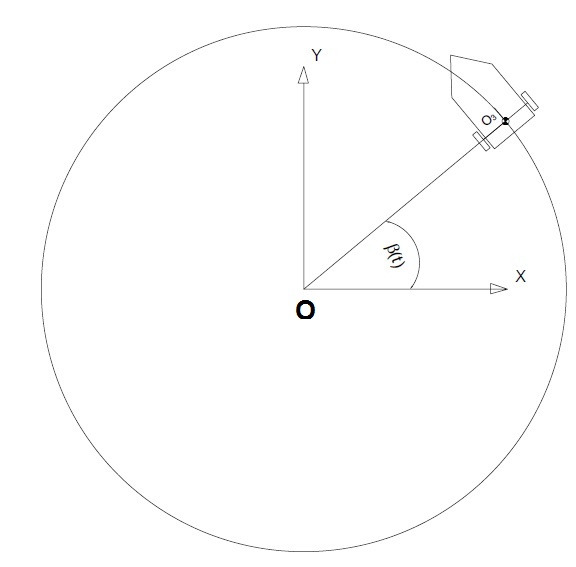
\includegraphics[height=250pt,keepaspectratio]{Chapter4/fig/pathCircle}
		\caption{Path Traced by Robot}
	\label{fig:CirTrace}
\end{figure}



\subsection{Inverse Dynamics}
Using the model inverse kinematic,  the wheel velocity and acceleration are determined using pseudo Inverse  % from the equation given below. Where $r$ is radius of the wheel and $\theta_i$ is the wheel roll angle of wheel \#1 and \#2. The platform angular velocity is $\omega$ and the Cartesian velocity of point o3 is given by $\dot{x},\dot{y}$ in body coordinate system %   
The wheel angle, velocity and acceleration were used in the dynamics equation  to calculate the torque required by each motor. The results are plotted in figure \ref{fig:spiral}. 

The equation of  dynamic model  is given in equation \ref{dnoc}, where the actuated joints are  $\theta_a(t)=(\theta_l, \theta_r) $ are the rear left and right wheel rotation angles. The dynamic  and kinematic  parameters used in the simulation is listed in table \ref{tb:massproperty}. The rear wheels $(i=1,2)$ and the platform $i=3$, twist $t_i^T=T_i\theta_a$, is given in equations \ref{twist1},\ref{twist2} and \ref{twist3}. The dynamic equation is of the vehicle on slope is given as 
\begin{equation}
\label{dnoc}
\begin{aligned}
T^TMT\ddot{\theta_a}&=-T^T(M\dot{T}+WMT)\dot{\theta_a}+T^T(w^J+w^G)\\
\text{where} \quad &
T=(T_1^T T_2^T T_3^T)^T, \quad M=diag(M_1, M_2, M_3)\\
T^TMT &=I_1+I_2+I_m+I_3= I_m+I_3\\
W&=diag(W_1,W_2,W_3),\quad w^G=g\sin\alpha, \quad \alpha=10^o
\end{aligned}
\end{equation}
$w^G$, $ w^J$ and $\alpha$ represent the gravitational force acting along the inclined  the external torque/Force applied by a motor and the inclination of the plane to horizontal respectively. The generalized inertia matrix $I_m$ and $I_3$ are given in \ref{eqn:I_wheel} and \ref{eqn:I_platform}.
As stated earlier the convective inertia term is zeros a the inertia matrices are constant. The motor torque  are then given a 
\begin{equation}
T1^Tw_1^j=\tau_1, \quad T_2^Tw_2^j=\tau_2
\end{equation}
\begin{equation}
 T_3^Tw^g=\begin{pmatrix}
\rho\delta k & r(\lambda i+(1/2)j) \\
 -\rho\delta k & r(-\lambda i+(1/2)j)
\end{pmatrix}
\begin{pmatrix}
0\\
-jg\sin\alpha
\end{pmatrix}=\begin{pmatrix}
-\frac{1}{2}rg\sin\alpha\\ -\frac{1}{2}rg\sin\alpha
\end{pmatrix}
\end{equation} 

The torques required at the wheels of the vehicle to  move up a spiral ramp  of slope $10^o$ and radius 5m is given figure \ref{fig:spiral}. 

 \begin{figure}
	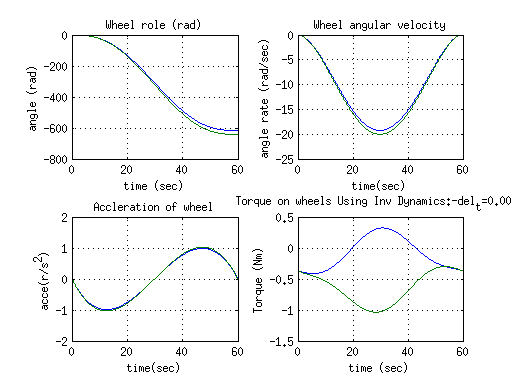
\includegraphics[height=300pt,keepaspectratio]{Chapter4/fig/FD}
	\captionof{figure}{Inverse dynamics of the mobile robot }
	\label{fig:spiral} 
\end{figure} 
%
\begin{table}[!htbp]
	\caption{Dynamic \& kinematic parameters }
	\label{tb:massproperty}
	\centering
	\begin{tabular}{l l l}
		\hline
		\emph{Part Name}  & \emph{ Property} & \emph{Value} \\
		\hline
		Rear Wheels  & mass &300g \\ 
		 & Moment of Inertia & diag(242, 242, 465)kg $mm^2$\\
		Base Frame & mass & 70Kg \\
		 & Moment Of Inertia & $ \begin{pmatrix}
		 1.18& 0.01&-0.05\\ 0.01 & 1.28 & 0.08\\
		 -0.05 & 0.08 & 0.53
		 \end{pmatrix} Kg-m^2$ \\
		   l & length & 400mm\\
		  r & wheel radius & 100mm\\
		 a & see figure &  \\ 
		\hline
		\end{tabular}
\end{table}
 
\section{Summary}
In this chapter the dynamic equation was derived for  the most general form of caster wheel configuration. Even though  only two caster wheel configuration was considered the same formulation can be extended to any number of caster wheels. It is shown that the  dynamics of standard caster wheels is a special case of the  general case with $d_1=0$.It is also proven why a caster needs  non-zero caster offset. There is a  need of extra actuator in case $d_2=0$.
    




